\documentclass[svgnames,11pt]{beamer}
\input{/home/tof/Documents/Cozy/latex-include/preambule_commun.tex}
\input{/home/tof/Documents/Cozy/latex-include/preambule_beamer.tex}
\usepackage{pgfpages} \setbeameroption{show notes on second screen=left}
\author[]{Christophe Viroulaud}
\title{Puissance 4\\Jeux de tests}
\date{\framebox{\textbf{Lang 09}}}
%\logo{}
\institute{Première - NSI}
\usetikzlibrary{shapes.multipart}

\begin{document}
\begin{frame}
    \note{\fcolorbox{black}{red}{{\LARGE puissance4-test-annexe.zip}}}
    \titlepage
\end{frame}
\begin{frame}
    \frametitle{}

    \begin{center}
        Le projet \emph{Puissance 4} est composé de plusieurs fichiers et contient de nombreuses fonctions.
    \end{center}

\end{frame}
\begin{frame}
    \frametitle{}

    \begin{framed}
        \centering Comment détecter les erreurs dans un programme informatique?
    \end{framed}

\end{frame}
\section{Cycle de vie d'un projet}
\begin{frame}
    \frametitle{Cycle de vie d'un projet}

    \begin{center}
        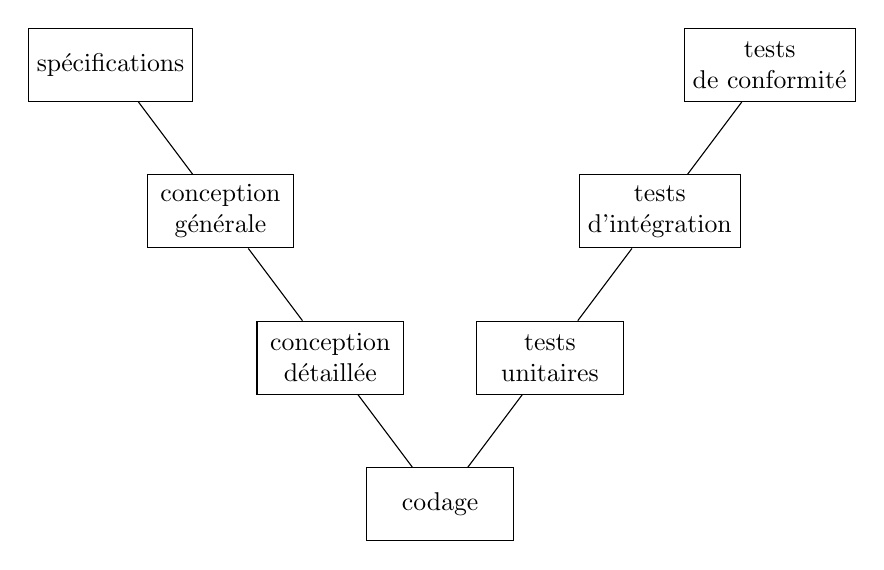
\begin{tikzpicture}[every text node part/.style={align=center}, scale=0.93,transform shape]
            \node[draw, minimum width=2cm, minimum height=1cm] (1) at(-4.5,6) {spécifications};
            \node[draw, minimum width=2cm, minimum height=1cm] (2) at(-3,4) {conception\\ générale};
            \node[draw, minimum width=2cm, minimum height=1cm] (3) at(-1.5,2) {conception\\ détaillée};
            \node[draw, minimum width=2cm, minimum height=1cm] (4) at(0,0) {codage};
            \node[draw, minimum width=2cm, minimum height=1cm] (5) at(1.5,2) {tests\\unitaires};
            \node[draw, minimum width=2cm, minimum height=1cm] (6) at(3,4) {tests\\d'intégration};
            \node[draw, minimum width=2cm, minimum height=1cm] (7) at(4.5,6) {tests\\de conformité};

            \draw (1) -- (2);
            \draw (2) -- (3);
            \draw (3) -- (4);
            \draw (4) -- (5);
            \draw (5) -- (6);
            \draw (6) -- (7);

        \end{tikzpicture}
    \end{center}

\end{frame}
\begin{frame}
    \frametitle{}

    \begin{center}
        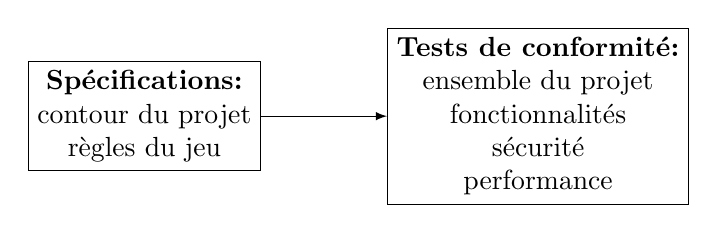
\begin{tikzpicture}[every text node part/.style={align=center}]
            \node[draw] (1) at(0,0) {\textbf{Spécifications:}\\contour du projet\\règles du jeu};
            \node[draw] (2) at (5,0) {\textbf{Tests de conformité:}\\ensemble du projet\\fonctionnalités\\sécurité\\performance};
            \draw[->,>=latex] (1) -- (2);
        \end{tikzpicture}
    \end{center}
    Exemple: Respect des règles du jeu
\end{frame}
\begin{frame}
    \frametitle{}

    \begin{center}
        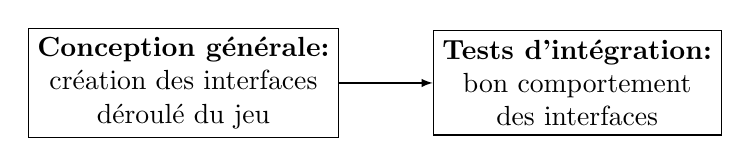
\begin{tikzpicture}[every text node part/.style={align=center}]
            \node[draw] (1) at(0,0) {\textbf{Conception générale:}\\création des interfaces\\déroulé du jeu};
            \node[draw] (2) at (5,0) {\textbf{Tests d'intégration:}\\bon comportement\\des interfaces};
            \draw[->,>=latex] (1) -- (2);
        \end{tikzpicture}
    \end{center}
    Exemple: Respect des différentes séquences du jeu (positionnement graphique du jeton\dots)
\end{frame}
\begin{frame}
    \frametitle{}

    \begin{center}
        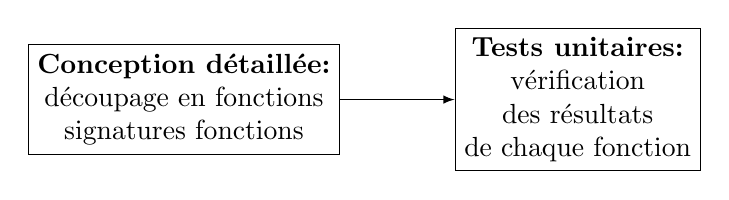
\begin{tikzpicture}[every text node part/.style={align=center}]
            \node[draw] (1) at(0,0) {\textbf{Conception détaillée:}\\découpage en fonctions\\signatures fonctions};
            \node[draw] (2) at (5,0) {\textbf{Tests unitaires:}\\vérification\\des résultats\\de chaque fonction};
            \draw[->,>=latex] (1) -- (2);
        \end{tikzpicture}
    \end{center}
    Exemple: Vérification de chaque fonction de calcul du gagnant (vertical, horizontal)
\end{frame}
\begin{frame}
    \frametitle{}

    \begin{aretenir}[]
        \begin{itemize}
            \item Un projet est découpé en plusieurs étapes.
            \item Chaque étape peut être réalisée par des équipes différentes.
            \item Les tests peuvent prendre plus de la moitié du temps de réalisation.
        \end{itemize}
    \end{aretenir}

\end{frame}
\section{Tests unitaires}
\subsection{Assertions}
\begin{frame}
    \frametitle{Test unitaires - assertions}

    \begin{aretenir}[Définition]
        \textbf{assertion:} Proposition que l'on avance et que l'on soutient comme vraie.
    \end{aretenir}

\end{frame}
\begin{frame}[fragile]
    \frametitle{}

    \begin{center}
        \begin{lstlisting}[language=Python , basicstyle=\ttfamily\small, xleftmargin=.2em, xrightmargin=-4em]
def placer_jeton(grille: list, colonne: int, joueur) -> int:
    ligne = tomber_ligne(grille, colonne)
    grille[ligne][colonne] = joueur
    return ligne
\end{lstlisting}
        \captionof{code}{Une fonction utile du Puissance 4}
        \label{CODE}
    \end{center}
    \textbf{Assertion:} la valeur de la colonne ne doit pas dépasser la largeur du plateau.
\end{frame}
\begin{frame}[fragile]
    \frametitle{}

    \begin{center}
        \begin{lstlisting}[language=Python , basicstyle=\ttfamily\small, xleftmargin=.2em, xrightmargin=-4em]
def placer_jeton(grille: list, colonne: int, joueur) -> int:

    assert colonne < LARGEUR, "La colonne est hors limite."

    ligne = tomber_ligne(grille, colonne)
    grille[ligne][colonne] = joueur
    return ligne
\end{lstlisting}
        \captionof{code}{Mise en place de l'assertion}
        \label{CODE}
    \end{center}
    \begin{aretenir}[]
        Si l'assertion est vérifiée la suite du code peut être exécutée. Sinon une \textbf{\texttt{AssertionError}} affiche un message.
    \end{aretenir}
\end{frame}
\begin{frame}[fragile]
    \frametitle{}

    Le fichier ne contient que des fonctions et pas de programme principal.
    \begin{center}
        \begin{lstlisting}[language=Python , basicstyle=\ttfamily\small, xleftmargin=2em, xrightmargin=2em]
if __name__ == "__main__":
    # provoque une erreur
    placer_jeton([], LARGEUR, 0)
\end{lstlisting}
        \captionof{code}{Tester la fonction dans le fichier.}
        \label{CODE}
    \end{center}
    \begin{aretenir}[Hors programme]
        La ligne
        \begin{lstlisting}[language=Python , basicstyle=\ttfamily\small, xleftmargin=2em, xrightmargin=2em]
if __name__ == "__main__":
\end{lstlisting}
        permet d'exécuter le programme principal uniquement si le fichier est exécuté directement (et pas importé).
    \end{aretenir}
\end{frame}
\begin{frame}
    \frametitle{}

    \begin{activite}
        \begin{enumerate}
            \item Télécharger et extraire le dossier compressé \textbf{\texttt{puissance4-test-annexe.zip}} sur le site \url{https://cviroulaud.github.io}
            \item Dans le fichier \textbf{\texttt{fonctions\_verif.py}} mettre en place des assertions dans la fonction \textbf{\texttt{verif\_gagnant}}. Elle permettront de vérifier que les paramètres \textbf{\texttt{ligne}} et \textbf{\texttt{colonne}} ne sortent pas de la taille du plateau de jeu.
        \end{enumerate}

    \end{activite}

\end{frame}
\begin{frame}[fragile]
    \frametitle{}
    \begin{center}
        \begin{lstlisting}[language=Python , basicstyle=\ttfamily\small, xleftmargin=1em, xrightmargin=-1em]
def verif_gagnant(grille: list, joueur: int, ligne: int, colonne: int) -> bool:

    assert ligne < HAUTEUR and ligne >= 0, "ligne hors limite"

    assert colonne < LARGEUR and colonne >= 0, "colonne hors limite"

# reste du code
\end{lstlisting}
    \end{center}
    \begin{center}
        \begin{lstlisting}[language=Python , basicstyle=\ttfamily\small, xleftmargin=2em, xrightmargin=2em]
if __name__ == "__main__":
    # provoque une erreur de ligne
    verif_gagnant([], 0, HAUTEUR, 0)
\end{lstlisting}
        \captionof{code}{Tester la fonction dans le fichier.}
        \label{CODE}
    \end{center}

\end{frame}

\subsection{Tests unitaires}
\begin{frame}
    \frametitle{Tests unitaires}

    Réaliser des tests externes pour:
    \begin{itemize}
        \item ne pas alourdir le code des fonctions,
        \item automatiser les tests.
    \end{itemize}

\end{frame}
\begin{frame}
    \frametitle{}
    Réaliser des tests externes pour:
    \begin{itemize}
        \item ne pas alourdir le code des fonctions,
        \item automatiser les tests.
    \end{itemize}
    \vspace{2cm}
    \begin{center}
        {\Large bibliothèque Python \textbf{\texttt{unittest}}}
    \end{center}

\end{frame}
\begin{frame}
    \frametitle{}

    \begin{aretenir}[Hors programme]
        La construction complète du fichier de tests n'est pas à maîtriser en classe de première.
    \end{aretenir}
    \begin{activite}
        Ouvrir le fichier \textbf{\texttt{tests\_placement.py}}
    \end{activite}
\end{frame}
\begin{frame}[fragile]
    \frametitle{}
    \begin{aretenir}[]
        Pour tester les fonctions il faut maîtriser les données de tests.
    \end{aretenir}
    \begin{center}
        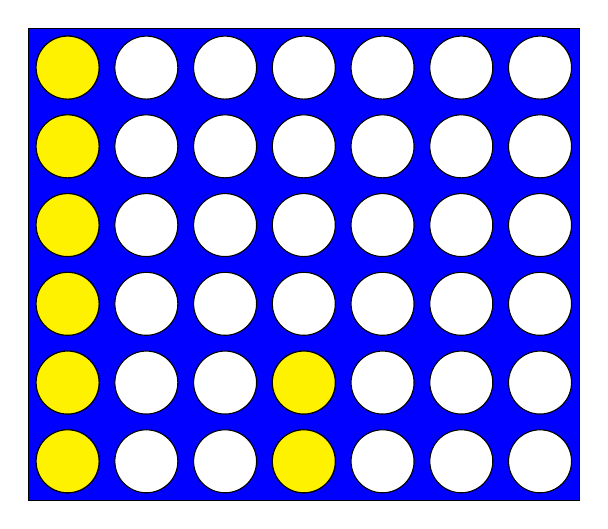
\begin{tikzpicture}
            \draw[fill=blue] (-.5,-.5)--(6.5,-.5)--(6.5,5.5)--(-.5,5.5)--cycle;
            \foreach \x in {0,1,...,6}{
                    \foreach \y in {0,1,...,5}{
                            \draw[fill=white] (\x,\y) circle (.4) ;
                        }
                }
            \foreach \y in {0,1,...,5}{
                    \draw[fill=yellow] (0,\y) circle (.4) ;
                }
                \foreach \y in {0,1}{
                    \draw[fill=yellow] (3,\y) circle (.4) ;
                }
        \end{tikzpicture}
    \end{center}
    


\end{frame}
\begin{frame}[fragile]
    \frametitle{}

    \begin{center}
        \begin{lstlisting}[language=Python , basicstyle=\ttfamily\small, xleftmargin=.5em, xrightmargin=-1em]
def setUp(self):
    """
    initialise la grille pour les tests
    """
    self.grille = [[VIDE for i in range(LARGEUR)] 
                            for j in range(HAUTEUR)]
\end{lstlisting}
        \captionof{code}{Initialiser des données pour les tests}
        \label{CODE}
    \end{center}   

\end{frame}
\begin{frame}[fragile]
    \frametitle{}
    \begin{center}
        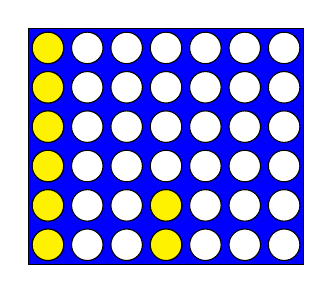
\begin{tikzpicture}[scale=.5]
            \draw[fill=blue] (-.5,-.5)--(6.5,-.5)--(6.5,5.5)--(-.5,5.5)--cycle;
            \foreach \x in {0,1,...,6}{
                    \foreach \y in {0,1,...,5}{
                            \draw[fill=white] (\x,\y) circle (.4) ;
                        }
                }
            \foreach \y in {0,1,...,5}{
                    \draw[fill=yellow] (0,\y) circle (.4) ;
                }
                \foreach \y in {0,1}{
                    \draw[fill=yellow] (3,\y) circle (.4) ;
                }
        \end{tikzpicture}
    \end{center}
        \begin{lstlisting}[language=Python , basicstyle=\ttfamily\small, xleftmargin=.5em, xrightmargin=-1em]
def setUp(self):
    """
    initialise la grille pour les tests
    """
    self.grille = [[VIDE for i in range(LARGEUR)] 
                            for j in range(HAUTEUR)]

    # rempli la première colonne
    for i in range(HAUTEUR):
        self.grille[i][0] = JAUNE
    # place 2 jetons dans colonne 3
    self.grille[5][3] = JAUNE
    self.grille[4][3] = JAUNE
\end{lstlisting}


\end{frame}
\begin{frame}[fragile]
    \frametitle{}

    \begin{center}
        \begin{lstlisting}[language=Python , basicstyle=\ttfamily\small, xleftmargin=1em, xrightmargin=1em]
def test_remplie(self):
    # test OK si renvoie est True
    self.assertTrue(est_remplie(self.grille, 0))
    # test OK si renvoie est False
    self.assertFalse(est_remplie(self.grille, 1))
\end{lstlisting}
        \captionof{code}{Réaliser des tests}
        \label{CODE}
    \end{center}

    \begin{aretenir}[Observations]
        \begin{itemize}
            \item La colonne 0 est pleine, la fonction doit renvoyer \textbf{\texttt{True}}.
            \item La colonne 1 est vide, la fonction doit renvoyer \textbf{\texttt{False}}.
        \end{itemize}
    \end{aretenir}
\end{frame}
\begin{frame}[fragile]
    \frametitle{}

    \begin{activite}
        En prenant modèle sur \textbf{\texttt{test\_remplie}} construire \textbf{\texttt{test\_tomber}} qui vérifie la position de jetons qu'on placerait en colonnes 0, 3 et 4.
        \\On pourra s'aider de la documentation: \url{https://tinyurl.com/doc-test}
    \end{activite}

    \begin{center}
        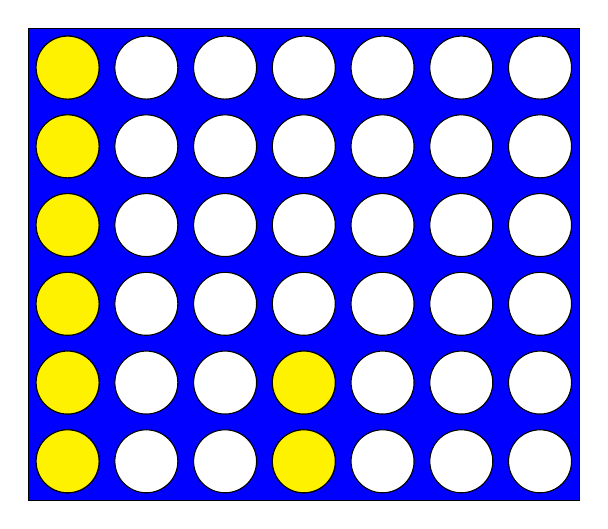
\begin{tikzpicture}
            \draw[fill=blue] (-.5,-.5)--(6.5,-.5)--(6.5,5.5)--(-.5,5.5)--cycle;
            \foreach \x in {0,1,...,6}{
                    \foreach \y in {0,1,...,5}{
                            \draw[fill=white] (\x,\y) circle (.4) ;
                        }
                }
            \foreach \y in {0,1,...,5}{
                    \draw[fill=yellow] (0,\y) circle (.4) ;
                }
                \foreach \y in {0,1}{
                    \draw[fill=yellow] (3,\y) circle (.4) ;
                }
        \end{tikzpicture}
    \end{center}
\end{frame}
\begin{frame}[fragile]
    \frametitle{Correction}

\begin{center}
\begin{lstlisting}[language=Python , basicstyle=\ttfamily\small, xleftmargin=.5em, xrightmargin=-1em]
def test_tomber(self):
    # jeton en colonne 4
    self.assertEqual(tomber_ligne(self.grille, 4), 5)
    # jeton en colonne 3
    self.assertEqual(tomber_ligne(self.grille, 3), 3)
    # jeton en colonne 0
    self.assertEqual(tomber_ligne(self.grille, 0), -1)
\end{lstlisting}
\end{center}   
\begin{aretenir}[Remarque]
Il est possible de créer un fichier de tests pour chaque fichier de fonctions.
\end{aretenir}
\end{frame}
\begin{frame}
    \frametitle{}

\begin{aretenir}[]
Les phases de tests sont une étape indispensable du cycle de vie d'un projet: elles permettent de maintenir la cohérence du code lors des modifications, ajouts\dots
\end{aretenir}   

\end{frame}
\end{document}